\documentclass{article}
\usepackage[dvipnames, table]{xcolor}
\usepackage[utf8]{inputenc}
\usepackage[dutch]{babel}
\usepackage{tabularx}
\usepackage{pdfpages}
\usepackage{enumitem}
\usepackage{geometry}
\geometry{
	a4paper,
	total={170mm,257mm},
	left=27mm,
	top=20mm,
}

\begin{document}
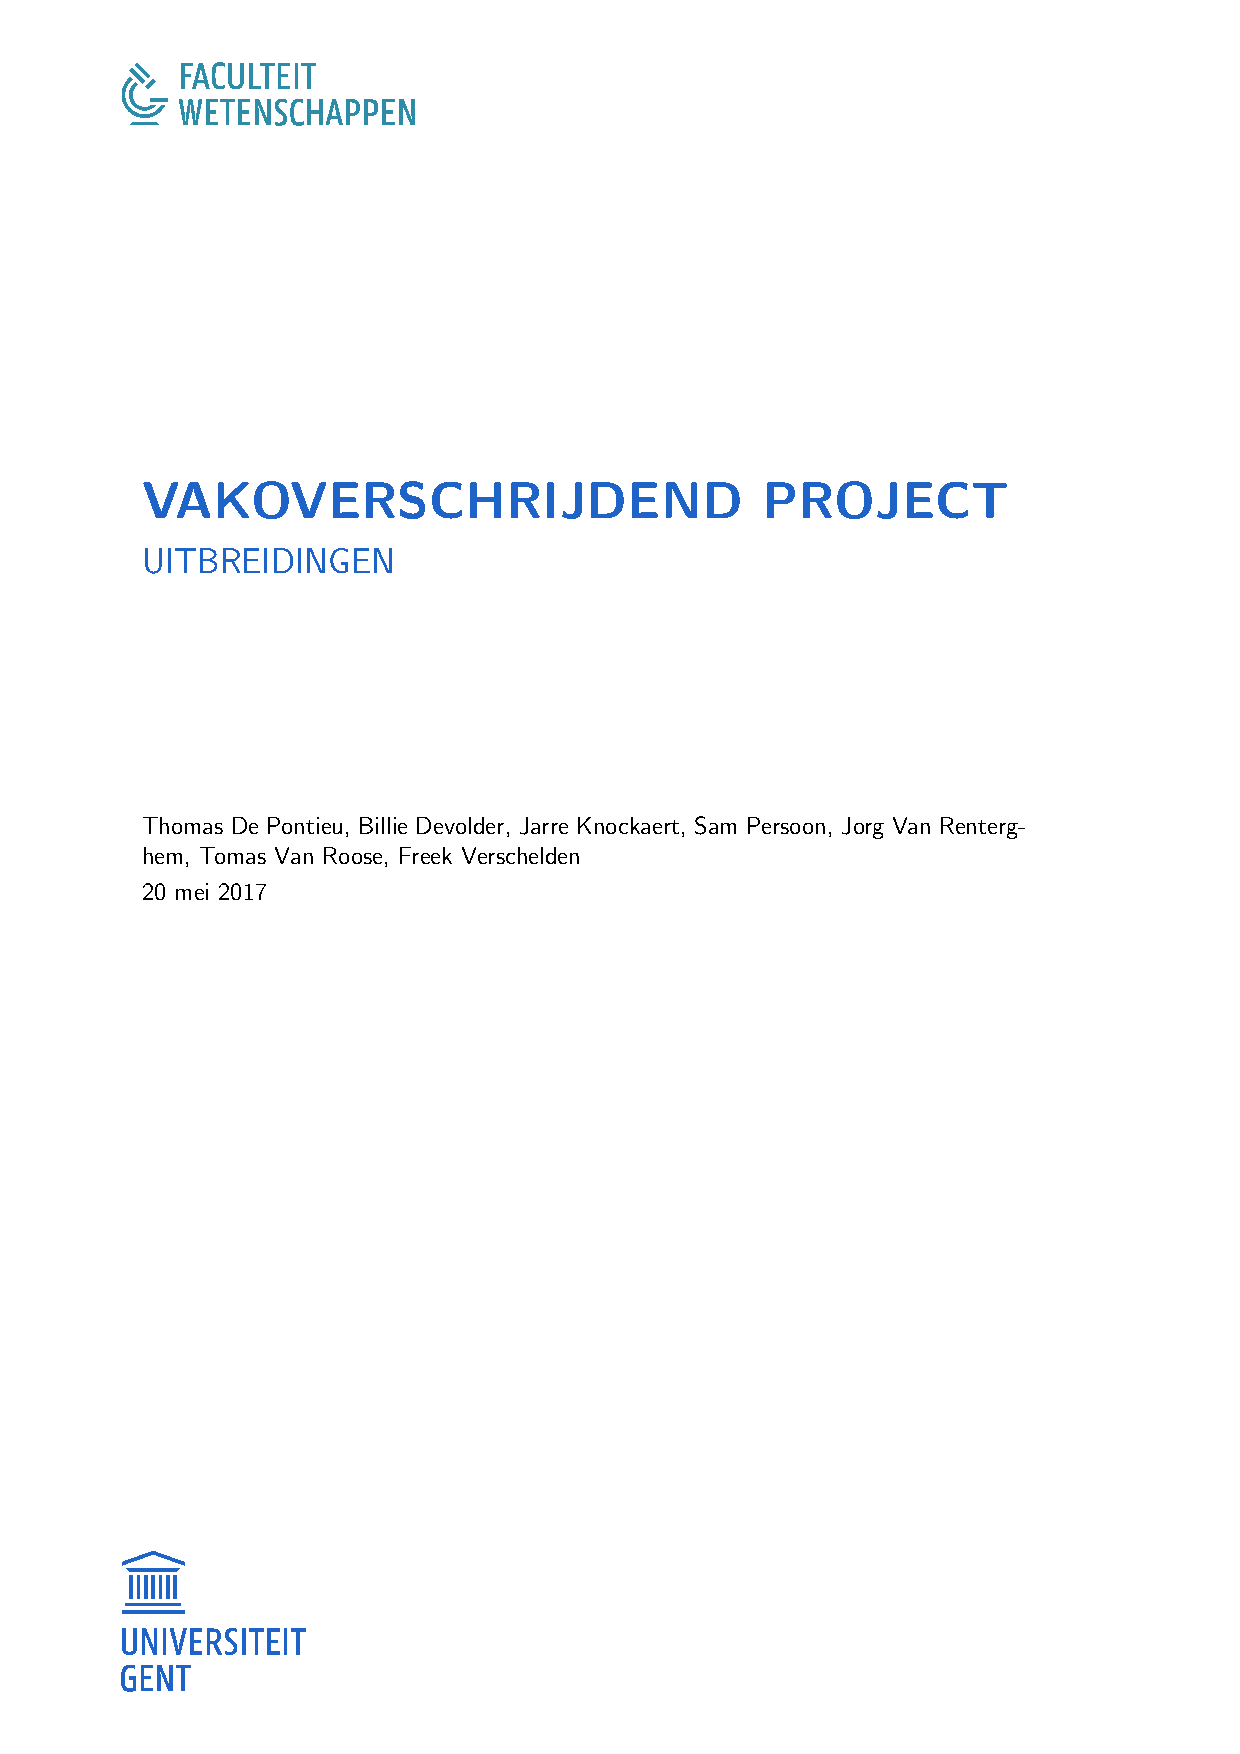
\includepdf[pages={1}]{voorblad.pdf}
\section{Vloten samenvoegen}

De eerste uitbreiding die we zullen bespreken is het samenvloegen van vloten. Indien 2 vestigingen van een bedrijf fuseren en de vloten moeten worden samengevoegd, zou het handig zijn dit met een simpele druk op een knop te kunnen doen. In principe moet er voor deze uitbreiding niets worden veranderd in de backend. De frontend kan alle voertuigen van een bepaalde vloot opvragen en dan via een PUT request de vloot veranderen van alle voertuigen in de vloot.
\\
\\
De aanpassingen staan hier zeker in verhouding tot de uitbreiding. In de backend en database moet er namelijk niets aangepast worden.

\section{Ondersteunen van boten}
	
Misschien wil Solvas, in een verre toekomst, zich ook gaan bezighouden met het verzekeren van boten. Hier nemen we aan dat het verzekeren van boten gebeurt op een gelijkaardige manier.
\\
\\
In het domeinmodel zou er een nieuwe klasse, \verb|WaterCraft|, moeten toegevoegd worden. Deze klasse zou een boot voorstellen en sterk lijken op de huidige klasse \verb|Vehicle|. Deze 2 klassen zouden grote gelijkenissen vertonen dus zou hier best een gemeenschappelijke superklasse voor gemaakt worden. In dit document zal deze superklasse \verb|AbstractVehicle| worden genoemd. De klasse \verb|Fleet| zou dan ook een collectie \verb|AbstractVehicle| objecten moeten hebben in plaats van \verb|Vehicle| objecten.
\\
\\
In de andere lagen moeten volgende zaken worden toegevoegd/veranderd:
\begin{enumerate}
	\item Er moet een hibernate mapping gemaakt worden voor de nieuwe klasse.
	\item Er moet een nieuw \verb|DataAccessObject| aangemaakt worden. Deze moet overerven van de abstracte klasse \verb|ProductionDAO|. In deze klasse moeten geen nieuwe methodes worden geïmplementeerd.
	\item Het nieuwe \verb|DataAccessObject| moet toegevoegd worden aan de \verb|DAOProvider|.
	\item Er moet een nieuwe \verb|Controller| worden aangemaakt die overerft van \verb|AbstractController|. In de nieuwe \verb|Controller| moet de isOwner function worden geïmplementeerd.
	\item De nieuwe \verb|Controller| moet worden toegevoegd aan de \verb|ControllerManager|.
	\item Er moet een \verb|RESTModel| worden aangemaakt voor de nieuwe klasse. Deze erft over van \verb|RESTAbstractModel|. In de klasse moet de constructor en de translate methode worden geïmplementeerd.
	\item Er moet een nieuwe \verb|RESTController| worden aangemaakt die overerft van \verb|RESTAbstractController|. Hier moet de getController methode worden geïmplementeerd een een methode die alle objecten, al dan niet gefilterd, teruggeeft.
\end{enumerate}

We denken dat de aanpassingen in verhouding staan tot de uitbreiding. Het meeste werk zou kruipen in het doorgeven van de waarden van de velden en deze te setten in de objecten. Dit is repetitief werk maar niet iets dat gemakkelijk te veralgemenen is. De meeste veranderingen in het domeinmodel zijn eenmalig. Indien er nog een ander soort voertuig zou bijkomen met andere velden, zou er enkel een klasse moeten worden toegevoegd die overerft van \verb|AbstractVehicle|.

\section{E-mails verzenden naar klanten bij bepaalde acties}

Voor het versturen van e-mails zouden we gebruik maken van het observer patroon. Als tussenklasse zouden we een \verb|EventBroker| gebruiken die events ontvangt en ze doorstuurt naar geregistreerde listeners. Dit is een singleton klasse. Onze controllers zouden bij elke actie een event genereren en doorgeven aan de \verb|EventBroker|. Hierdoor blijven de controller module en e-mail module volledig ontkoppeld. De controllers kunnen eenvoudig aangepast geworden. Enkel \verb|AbstractController| zal moeten worden aangepast. De e-mail module zou een listener worden. Aan de hand van de informatie die wordt doorgestuurd bij een event kan er dan beslist worden of er al dan niet een e-mail moet verstuurd worden.

\section{Algemene log tonen}

Er zou in de applicatie ook een algemene log kunnen getoond worden. Bij het ontwerpen van het logsysteem hebben we hier rekening mee gehouden dus kan dit relatief gemakkelijk worden toegevoegd. Bij de \verb|LogEntryController| moet een methode worden aangemaakt die alle logs ophaalt van de \verb|LogEntryDAO|. Bij \verb|RESTLogEntryController| moet een methode worden aangemaakt die de methode van \verb|LogEntryController| oproept.

\section{Ondersteunen van andere soorten correcties}

Indien we andere soorten correcties willen ondersteunen, moet er bij het veranderen van een \verb|VehicleInsurance|, naast het object zelf, ook de datum waarop de verandering moet plaatsvinden worden meegegeven.  Voor de API call wordt er best een wrapper object aangemaakt die de datum en de \verb|RESTVehicleInsurance| bevat. Bij de put methode van \verb|VehicleInsuranceController| zal nu ook de datum moeten worden meegegeven. De code die moet gebruikt worden voor het genereren van correcties kan grotendeels hergebruikt worden van de andere soorten correcties (verzekering toevoegen en verwijderen).

\section{Exporteren van voertuigen}

Voor deze uitbreiding moeten we de bestaande code niet aanpassen maar gewoon code toevoegen. Ten eerste hebben we hier een nieuwe API call voor nodig. In de methode die de API call implementeert, zullen de voertuigen moeten worden opgehaald aan de hand van de \verb|VehicleController|. We zullen ook een nieuwe module moeten implementeren die een xls bestand kan aanmaken. Deze module zal ergens een methode nodig hebben waar de lijst van voertuigen aan moet worden meegegeven en die een bestand teruggeeft. De methode die de API call implementeert, zal dan deze nieuwe methode oproepen en het bestand teruggeven. Hier staan de aanpassingen in verhouding tot de uitbreiding: aan de bestaande code moet niets aangepast worden. 
\end{document}
